\documentclass[tikz,border=4pt]{standalone}
% Estilo común de los diagramas de bloques (se usa con \input en cada standalone)
\usepackage[defaultsans,scale=0.92]{lato}
\usepackage{libertinust1math}
\usepackage{xcolor,amsmath}
\usepackage{tikz}
\usetikzlibrary{positioning,arrows.meta,calc,shapes.geometric}
\usepackage{../../notacion}
\definecolor{ctrlazul}{HTML}{1E5AA8}\definecolor{ctrlnoche}{HTML}{14213D}
\definecolor{ctrlcoral}{HTML}{D1495B}\definecolor{ctrlverde}{HTML}{2A9D8F}
\definecolor{ctrlambar}{HTML}{E09F3E}\definecolor{ctrlgris}{HTML}{5C677D}
\definecolor{ctrlvioleta}{HTML}{6C4AB6}\definecolor{ctrlteal}{HTML}{0F7173}
\tikzset{
  >={Stealth[length=2.4mm]}, every node/.style={font=\small},
  bloque/.style={draw=ctrlnoche,fill=ctrlazul!7,thick,rounded corners=1.5pt,minimum height=9mm,minimum width=13mm,inner sep=4pt},
  suma/.style={draw=ctrlnoche,thick,circle,inner sep=0pt,minimum size=6mm},
  senal/.style={->,thick,draw=ctrlnoche},
  rot/.style={font=\footnotesize,text=ctrlgris},
}

\begin{document}
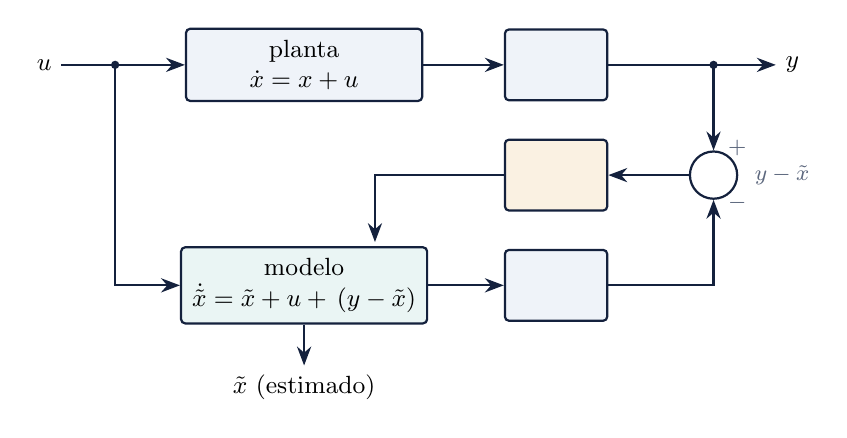
\begin{tikzpicture}
  \node (u) at (-3.3,0) {$u$};
  \node[bloque,minimum width=30mm,align=center] (P) at (0,0) {planta\\ $\dot x=\Am x+\Bm u$};
  \node[bloque] (C) at (3.2,0) {$\Cm$};
  \node (y) at (6.2,0) {$y$};
  \node[bloque,minimum width=30mm,fill=ctrlverde!10,align=center] (O) at (0,-2.8) {modelo\\ $\dot{\tilde x}=\Am\tilde x+\Bm u+\Lm\,(y-\Cm\tilde x)$};
  \node[bloque] (Co) at (3.2,-2.8) {$\Cm$};
  \node[suma] (S) at (5.2,-1.4) {};
  \node[bloque,fill=ctrlambar!15] (L) at (3.2,-1.4) {$\Lm$};
  \node (xt) at (0,-4.1) {$\tilde x$ (estimado)};
  \coordinate (nu) at (-2.4,0); \coordinate (ny) at (5.2,0);
  \draw[senal] (u)--(P); \fill[ctrlnoche] (nu) circle (1.5pt); \draw[senal] (nu)|-(O.west);
  \draw[senal] (P)--(C); \draw[senal] (C)--(y); \fill[ctrlnoche] (ny) circle (1.5pt);
  \draw[senal] (ny)--(S); \draw[senal] (O)--(Co); \draw[senal] (Co)-|(S);
  \draw[senal] (S)--(L); \draw[senal] (L.west)-|(0.9,-2.25);
  \node[rot] at ($(S)+(3mm,-3.5mm)$) {$-$}; \node[rot] at ($(S)+(3mm,3.5mm)$) {$+$};
  \draw[senal] (O)--(xt);
  \node[rot,anchor=west] at ($(S)+(4mm,0)$) {$y-\Cm\tilde x$};
\end{tikzpicture}
\end{document}
